% !TEX program = xelatex
\documentclass[UTF8,fontset=fandol,a4paper,11pt]{ctexart}
\usepackage[margin=21mm,top=23mm,bottom=22mm,headheight=16pt]{geometry}
\usepackage{amsmath,amssymb,mathtools,bm}
\usepackage{tikz}
\usetikzlibrary{arrows.meta,calc,angles,quotes,patterns}
\usepackage{xcolor,booktabs,array,longtable,enumitem,fancyhdr,needspace}
\usepackage[unicode,hidelinks]{hyperref}
\definecolor{ink}{HTML}{24343C}
\definecolor{accent}{HTML}{166A70}
\definecolor{muted}{HTML}{65747A}
\definecolor{rulegray}{HTML}{D4DDE0}
\definecolor{warm}{HTML}{966037}
\color{ink}
\setlength{\parindent}{2em}
\setlength{\parskip}{4pt}
\linespread{1.12}
\AtBeginDocument{\setlength{\abovedisplayskip}{6pt plus 2pt minus 1pt}
\setlength{\belowdisplayskip}{6pt plus 2pt minus 1pt}
\setlength{\abovedisplayshortskip}{0pt plus 1pt}
\setlength{\belowdisplayshortskip}{4pt plus 1pt}}
\setlist[enumerate]{label=(\arabic*),leftmargin=2.3em,itemsep=3pt,topsep=4pt}
\setlist[itemize]{leftmargin=2em,itemsep=2pt,topsep=4pt}
\allowdisplaybreaks[1]
\setlength{\emergencystretch}{2em}
\setcounter{secnumdepth}{0}
\providecommand{\tightlist}{\setlength{\itemsep}{0pt}\setlength{\parskip}{0pt}}
\ctexset{section={format=\Large\bfseries\color{accent},beforeskip=10pt,afterskip=9pt},
subsection={format=\normalsize\bfseries\color{accent},beforeskip=10pt,afterskip=4pt},
subsubsection={format=\normalsize\bfseries,beforeskip=8pt,afterskip=3pt}}
\pagestyle{fancy}
\fancyhf{}
\fancyhead[L]{\small\color{muted}物理学难题集萃}
% 页眉仅保留书名；版本名称只在封面显示。
\fancyfoot[L]{\small\color{muted}\chapterlabel}
\fancyfoot[R]{\small\thepage}
\renewcommand{\headrulewidth}{0.4pt}
\renewcommand{\footrulewidth}{0pt}
\newcommand{\dd}{\mathop{}\!\mathrm{d}}
\newcommand{\vect}[1]{\bm{#1}}
\newcommand{\tagline}[1]{\noindent{\small\color{muted}#1}\par}
\newcommand{\result}[1]{\begin{equation*}\boxed{#1}\end{equation*}}
\newcommand{\figcaption}[1]{\par\vspace{2pt}{\small\color{muted}#1}\par}
\newcommand{\teach}[2]{\Needspace{4\baselineskip}\subsection*{讲解要点与追问}#1\par\smallskip\noindent\textbf{追问：}#2\par}
\newcommand{\workarea}{\par\vspace{7mm}\noindent{\small\color{muted}作答区}\par\vspace{4mm}
\noindent\textcolor{rulegray}{\rule{\linewidth}{0.3pt}}\par\vspace{16mm}
\noindent\textcolor{rulegray}{\rule{\linewidth}{0.3pt}}\par\vspace{16mm}
\noindent\textcolor{rulegray}{\rule{\linewidth}{0.3pt}}\par\vspace{16mm}
\noindent\textcolor{rulegray}{\rule{\linewidth}{0.3pt}}}
\tikzset{axis/.style={-{Stealth[length=2mm]},thin,color=muted},
motion/.style={-{Stealth[length=2.3mm]},thick,color=accent},
force/.style={-{Stealth[length=2.3mm]},thick,color=warm},
traj/.style={thick,color=accent},guide/.style={dashed,thin,color=muted},
object/.style={thick,color=ink},every node/.style={font=\small}}\widowpenalty=10000\clubpenalty=10000\displaywidowpenalty=10000\newcommand{\chapterlabel}{电磁学第三章\quad 电磁感应}



\hypersetup{pdftitle={电磁学第三章 电磁感应·学生版},pdfauthor={}}

\begin{document}

\pdfbookmark[0]{电磁学第三章 电磁感应}{cover}

\thispagestyle{empty}\vspace*{22mm}
\noindent{\Huge\bfseries 物理学难题集萃}\par\vspace{10mm}
\noindent{\LARGE 电磁学第三章}\par\vspace{6mm}
\noindent{\LARGE 电磁感应}\par\vspace{12mm}
\noindent{\Large\color{accent}学生版}\par\vspace{9mm}
\noindent\textcolor{accent}{\rule{\linewidth}{1pt}}\par\vspace{9mm}
\noindent 共22题\par\vfill\clearpage
\pdfbookmark[1]{题目目录}{contents}\section*{题目目录}
\begin{longtable}{@{}r p{113mm} r@{}}\toprule 题号 & 题目 & 页码\\\midrule

\hyperref[q:1]{1} & \hyperref[q:1]{三角形线框旋转时的平均电流} & \pageref{q:1} \\

\hyperref[q:2]{2} & \hyperref[q:2]{恒力收缩导线圆圈的闭合时间} & \pageref{q:2} \\

\hyperref[q:3]{3} & \hyperref[q:3]{铜环倾倒时的磁阻尼与能量} & \pageref{q:3} \\

\hyperref[q:4]{4} & \hyperref[q:4]{翻转线圈测地磁场的分支判断} & \pageref{q:4} \\

\hyperref[q:5]{5} & \hyperref[q:5]{双格线框移出磁场的外力功} & \pageref{q:5} \\

\hyperref[q:6]{6} & \hyperref[q:6]{双导体棒的速度趋同与间距上限} & \pageref{q:6} \\

\hyperref[q:7]{7} & \hyperref[q:7]{强磁场中下落薄圆盘的电磁惯性} & \pageref{q:7} \\

\hyperref[q:8]{8} & \hyperref[q:8]{随动电压表与圆弧导体的端点电势} & \pageref{q:8} \\

\hyperref[q:10]{10} & \hyperref[q:10]{磁流体发电机的流速反馈} & \pageref{q:10} \\

\hyperref[q:11]{11} & \hyperref[q:11]{双辐条轮的电磁传动与效率} & \pageref{q:11} \\

\hyperref[q:12]{12} & \hyperref[q:12]{感生电场中的圆弧与三角形混合电路} & \pageref{q:12} \\

\hyperref[q:13]{13} & \hyperref[q:13]{交变磁场中圆柱的涡流热功率} & \pageref{q:13} \\

\hyperref[q:14]{14} & \hyperref[q:14]{电压表引线路径与感生电压} & \pageref{q:14} \\

\hyperref[q:15]{15} & \hyperref[q:15]{增长磁场中圆形导轨上的带电珠} & \pageref{q:15} \\

\hyperref[q:16]{16} & \hyperref[q:16]{螺线管断电时带电圆盘的转动} & \pageref{q:16} \\

\hyperref[q:17]{17} & \hyperref[q:17]{偏心感生电场驱动细管中的简谐运动} & \pageref{q:17} \\

\hyperref[q:18]{18} & \hyperref[q:18]{无电阻线框穿越窄磁场带的分段运动} & \pageref{q:18} \\

\hyperref[q:19]{19} & \hyperref[q:19]{由持久电流衰减估计电阻率上限} & \pageref{q:19} \\

\hyperref[q:20]{20} & \hyperref[q:20]{恒流双线分离时的磁能与机械功} & \pageref{q:20} \\

\hyperref[q:21]{21} & \hyperref[q:21]{柔性线圈测量磁场线积分} & \pageref{q:21} \\

\hyperref[q:22]{22} & \hyperref[q:22]{相切圆环与反向双直线电流的互感} & \pageref{q:22} \\

\hyperref[q:23]{23} & \hyperref[q:23]{互感线圈的短接、串联与并联} & \pageref{q:23} \\

\bottomrule\end{longtable}

本章采用SI单位。磁通量的正方向由回路方向按右手定则确定；$\odot$表示垂直纸面向外，$\otimes$表示垂直纸面向里。净电量$\int I\dd t$与累计电量$\int|I|\dd t$分别说明。除题目明确保留自感外，感应电流采用电阻主导的准稳态近似。

\clearpage

\pdfbookmark[2]{第 1 题 三角形线框旋转时的平均电流}{q1}

\section*{第 1 题\quad 三角形线框旋转时的平均电流}\label{q:1}

边长为$a$的等边三角形磁场区域内，匀强磁场$B$垂直纸面向外，区域外磁场为零。边长同为$a$、总电阻为$R$的等边三角形导体框架$ABC$，在$t=0$与磁场边界重合，随后以周期$T$绕共同中心在纸面内顺时针匀速转动。按$A\to B\to C\to A$流动的电流为正，忽略自感。求$0\le t\le T/6$及$0\le t\le T/2$内的平均电流$\overline I_1,\overline I_2$。

\begin{center}\begin{minipage}{.98\linewidth}\centering
\begin{tikzpicture}[scale=.85]

\fill[accent!8] (90:2)--(210:2)--(330:2)--cycle;
\draw[object] (90:2) node[above]{$A$}--(210:2) node[below left]{$B$}--(330:2) node[below right]{$C$}--cycle;
\draw[guide] (0,0)--(90:2);\fill (0,0) circle(1.4pt) node[left]{$O$};
\node at (0,.7){$\odot\ B$};\draw[motion] (55:2.35) arc(55:-15:2.35) node[right]{顺时针};
\node at (0,-2.05){$t=0$，框与场区重合};\draw[<->] (-1.73,-1.3)--(1.73,-1.3) node[midway,below]{$a$};

\end{tikzpicture}\figcaption{图电3.1\quad 固定三角形场区与初始线框。}\end{minipage}\end{center}

\workarea

\clearpage

\pdfbookmark[2]{第 2 题 恒力收缩导线圆圈的闭合时间}{q2}

\section*{第 2 题\quad 恒力收缩导线圆圈的闭合时间}\label{q:2}

柔软导体回路$ABCDA$的总电阻恒为$R$，其中$AB$段的一部分绕成初始半径$r_0$的圆圈，圆圈处于垂直其平面的匀强磁场$B$中。$B$端固定，$C,D$端自由；沿$BA$方向对$A$端施加恒力$F$，使圆圈缓慢缩小并始终保持圆形。忽略导线惯性、自感、弹性储能和一切机械阻力，圆圈以外部分的磁通变化忽略不计。求半径缩至零的形式闭合时间$T$。

\begin{center}\begin{minipage}{.98\linewidth}\centering
\begin{tikzpicture}[scale=.85]

\draw[object] (-2,1.8) node[above left]{$B$（固定）}--(-.65,1.8)
.. controls(-.4,1.8) and(-.45,1.15)..(.17365,.98481)
arc(80:-260:1)
.. controls(.05,1.15) and(.35,1.8)..(.65,1.8)--(3.8,1.8) node[above]{$A$};
\draw[object] (3.8,1.8)--(3.8,-1.5) node[right]{$D$}--(-2,-1.5) node[left]{$C$}--(-2,1.8);
\draw[force] (4.1,1.8)--(5.4,1.8) node[right]{$F$};
\draw[axis] (0,0)--(-.707,-.707) node[midway,below]{$r_0$};\node at(.3,.2){$\odot B$};

\end{tikzpicture}\figcaption{图电3.2\quad 圆圈串在$AB$软线段中，交叉处不电接触；外部回路示意。}\end{minipage}\end{center}

\workarea

\clearpage

\pdfbookmark[2]{第 3 题 铜环倾倒时的磁阻尼与能量}{q3}

\section*{第 3 题\quad 铜环倾倒时的磁阻尼与能量}\label{q:3}

细铜圆环的主半径$r_1=1.0\,\mathrm{cm}$，圆形导线截面半径$r_2=1.0\,\mathrm{mm}$。圆环竖放，底部有光滑固定栓限制滑动，使它可绕经过最低点的水平切线轴倾倒。竖直向上匀强磁场$B=1.0\,\mathrm T$。圆环由与竖直方向夹角$\theta_0=1.0\,\mathrm{rad}$的位置静止释放，最后到达水平位置。铜的电导率$\sigma=6.25\times10^7\,\mathrm{S/m}$，密度$\rho=8.93\times10^3\,\mathrm{kg/m^3}$，取$g=9.80\,\mathrm{m/s^2}$，忽略自感、空气阻力及接触耗散。
\begin{enumerate}
\item 通过估算和能量关系，判断重力势能如何分配；说明平均转速能否直接估计倒地瞬间的转动动能。
\item 在忽略角加速度项的准静态近似中，令磁阻力矩与重力矩相等，求从一般初始角$0<\theta_0<\pi/2$到水平位置的时间，并计算$\theta_0=1.0\,\mathrm{rad}$的结果。讨论近似的适用范围。
\end{enumerate}

\begin{center}\begin{minipage}{.98\linewidth}\centering
\begin{tikzpicture}[scale=.85]

\draw[object] (-1,0)--(3.2,0);\fill(0,0) circle(2pt) node[below]{$P$（栓轴）};
\draw[guide] (0,0)--(0,2.8);\draw[object,very thick] (0,0)--(2.6927,1.7290);
\fill(1.3464,.8645) circle(2pt) node[above]{$G$};\node at(.65,.18){$r_1$};
\draw (0,.85) arc(90:32.7042:.85);\node at(.48,1.02){$\theta_0$};
\foreach \x in {4,4.7,5.4}{\draw[motion] (\x,.2)--(\x,2.8);}\node at(4.7,3.2){$B$};
\node at(-.9,2.3){侧视};\node at(7.5,2.2){导线截面};\draw[object] (7.5,1.1) circle(.4);
\draw[axis] (7.5,1.1)--(7.9,1.1) node[midway,above]{$r_2$};

\end{tikzpicture}\figcaption{图电3.3\quad 初始环面倾角为$1.0\,\mathrm{rad}$；重心$G$距栓轴为$r_1$。}\end{minipage}\end{center}

\workarea

\clearpage

\pdfbookmark[2]{第 4 题 翻转线圈测地磁场的分支判断}{q4}

\section*{第 4 题\quad 翻转线圈测地磁场的分支判断}\label{q:4}

水平桌面上有矩形线圈$abcd$，$ab=\ell_1$指向北方，$bc=\ell_2$沿东西方向，总电阻为$R$，面积$S=\ell_1\ell_2$。先绕南北方向的中心轴翻转$180^\circ$，使$ab$与$cd$交换位置，测得通过导线的净电量绝对值为$Q_1$。再固定南侧的$ad$边，将北侧边抬起$90^\circ$使线圈竖直；线圈从水平状态的向上法线转向南方，测得这次净电量绝对值为$Q_2$。地磁场的水平分量向北，竖直分量可向上或向下。忽略自感。
求地磁场大小的可能值及各分支的条件；说明还需记录什么信息才能消除歧义。净电量指$\int I\dd t$，不等同于累计电量$\int|I|\dd t$。

\begin{center}\begin{minipage}{.98\linewidth}\centering
\begin{tikzpicture}[scale=.85]

\draw[object] (0,0) node[below left]{$a$}--(0,2.5) node[above left]{$b$}--(4,2.5) node[above right]{$c$}--(4,0) node[below right]{$d$}--cycle;
\draw[axis] (5,0)--(5,2) node[above]{北};\draw[axis] (5,0)--(6.5,0) node[right]{东};
\draw[<->] (-.5,0)--(-.5,2.5) node[midway,left]{$\ell_1$};\draw[<->] (0,-.6)--(4,-.6) node[midway,below]{$\ell_2$};
\draw[guide] (2,-.2)--(2,2.9);\node at(2,4){先绕南北轴翻转$180^\circ$};
\draw[motion] (.5,2.8)--(.5,3.4);\node at(5.7,3.4){再抬北边};

\end{tikzpicture}\figcaption{图电3.4\quad 俯视矩形及两次操作，第二步固定南边$ad$。}\end{minipage}\end{center}

\workarea

\clearpage

\pdfbookmark[2]{第 5 题 双格线框移出磁场的外力功}{q5}

\section*{第 5 题\quad 双格线框移出磁场的外力功}\label{q:5}

“日”字形闭合导线框$abcdef$如图，$a,f,e$在上边，$b,c,d$在下边，三条竖边$ab,fc,ed$等长，$ab=bc=cd=de=ef=fa=\ell=0.10\,\mathrm m$。$ab,fc,de$的电阻均为$R=3.0\,\Omega$，$cd,fe$均为$r=1.5\,\Omega$，$bc,af$电阻忽略。线框起初全部位于$B=1.0\,\mathrm T$的匀强磁场内，磁场垂直框面向里，右侧直边界与$de$平行。以$v=24\,\mathrm{m/s}$向右匀速拉出整个线框，忽略自感。求拉力做的总功。

\begin{center}\begin{minipage}{.98\linewidth}\centering
\begin{tikzpicture}[scale=.85]

\fill[accent!7] (-.7,-.5) rectangle (4.1,3.3);\draw[guide] (4.1,-.5)--(4.1,3.3) node[above]{场区边界};
\draw[object] (0,0) node[below]{$b$}--(0,2.4) node[above]{$a$}--(2.4,2.4) node[above]{$f$}--(4.8,2.4) node[above]{$e$}--(4.8,0) node[below]{$d$}--(2.4,0) node[below]{$c$}--cycle;
\draw[object] (2.4,0)--(2.4,2.4);\node[left] at(0,1.2){$R$};\node[right] at(2.4,1.2){$R$};\node[right] at(4.8,1.2){$R$};
\node[above] at(3.6,2.4){$r$};\node[below] at(3.6,0){$r$};\node at(1,1.2){$\otimes B$};
\draw[motion] (5.5,1.2)--(6.7,1.2) node[right]{$v$};

\end{tikzpicture}\figcaption{图电3.5\quad 两格均为边长$\ell$的正方形；图示右边已离开场区。}\end{minipage}\end{center}

\workarea

\clearpage

\pdfbookmark[2]{第 6 题 双导体棒的速度趋同与间距上限}{q6}

\section*{第 6 题\quad 双导体棒的速度趋同与间距上限}\label{q:6}

水平面内有两条足够长的光滑平行理想导轨，间距为$\ell$，处于垂直纸面向里的匀强磁场$B$中。两根相同导体棒跨接在导轨上，每根长$\ell$、质量$m$、电阻$R$，组成闭合回路。忽略自感，初始左棒静止、右棒以$v_0$向右运动。求右棒速度$v_1(t)$和两棒间距增加量$x(t)$及其上限。

\begin{center}\begin{minipage}{.98\linewidth}\centering
\begin{tikzpicture}[scale=.85]

\draw[object] (-1,0)--(6,0) (-1,2.4)--(6,2.4);
\draw[object,very thick] (0,0)--(0,2.4) (4,0)--(4,2.4);
\node[left] at(0,1.2){$m,R$};\node[right] at(4,1.2){$m,R$};\node at(2,1.2){$\otimes B$};
\draw[motion] (4,2.8)--(5.4,2.8) node[right]{$v_0$};\node at(0,3){初始静止};
\draw[<->] (-1.4,0)--(-1.4,2.4) node[midway,left]{$\ell$};

\end{tikzpicture}\figcaption{图电3.6\quad 两棒与理想导轨形成总电阻$2R$的回路。}\end{minipage}\end{center}

\workarea

\clearpage

\pdfbookmark[2]{第 7 题 强磁场中下落薄圆盘的电磁惯性}{q7}

\section*{第 7 题\quad 强磁场中下落薄圆盘的电磁惯性}\label{q:7}

半径为$R$、厚度为$D$的金属薄圆盘，盘面竖直，匀强磁场$B$沿水平方向且平行于盘面。圆盘由静止自由下落，密度$\rho=9.0\times10^3\,\mathrm{kg/m^3}$，电阻率视为零，忽略空气阻力和边缘效应，$D\ll R$。求使下落加速度较$g$减小$0.1\%$所需磁感应强度的数量级。取$\varepsilon_0=8.85\times10^{-12}\,\mathrm{F/m}$。

\begin{center}\begin{minipage}{.98\linewidth}\centering
\begin{tikzpicture}[scale=.85]

\draw[object] (0,0) circle(1.5);\draw[axis] (0,0)--(1.05,1.05) node[midway,above left]{$R$};
\draw[motion] (-2,0)--(2.1,0) node[right]{$B$};\draw[motion] (0,-1.8)--(0,-2.8) node[right]{$v,a$};
\node at(4.5,1){盘面竖直，厚度$D$};\node at(4.5,-.7){$B,v$均在盘面内};

\end{tikzpicture}\figcaption{图电3.7\quad 正视圆盘；电荷分离沿垂直盘面的厚度方向。}\end{minipage}\end{center}

\workarea

\clearpage

\pdfbookmark[2]{第 8 题 随动电压表与圆弧导体的端点电势}{q8}

\section*{第 8 题\quad 随动电压表与圆弧导体的端点电势}\label{q:8}

一块沿$x$方向无限长、宽为$L$的静止金属板电阻可忽略。半径$L/\sqrt2$的圆弧导体$aebcfd$沿板的长边以速度$v$滑动，圆弧平面垂直$x$轴，$a,d$始终接触板的两条边。正视图中$a,b,c,d$是圆上内接正方形的左下、左上、右上、右下顶点，$e,f$为圆的最左、最右点；$ae,eb,cf,fd$各为八分之一圆弧、电阻均为$R/2$，$bc$为四分之一圆弧、电阻为$R$。匀强磁场$B$竖直向上。电阻$R_V=nR$的电压表位于圆心$O$，由理想径向导线连接$b,c$，并随圆弧一起运动，$n>0$。求电压表读数及静电势差$U_e-U_f$。

\begin{center}\begin{minipage}{.98\linewidth}\centering
\begin{tikzpicture}[scale=.85]

\draw[guide] (-1.5,-1.5)--(1.5,-1.5);\draw[object] (-1.5,-1.5) arc(225:-45:2.1213);
\draw[object] (-1.5,1.5)--(0,0)--(1.5,1.5);\draw[fill=white] (0,0) circle(.23) node{$V$};
\foreach \x/\y/\lab/\pos in {-1.5/-1.5/a/below left,-1.5/1.5/b/above left,1.5/1.5/c/above right,1.5/-1.5/d/below right,-2.121/0/e/left,2.121/0/f/right}{\fill (\x,\y) circle(1.2pt) node[\pos]{$\lab$};}
\draw[object] (-1.5,-1.5)--(-.4,-2.5)--(2.6,-2.5)--(1.5,-1.5);\node at(1.1,-2.8){静止金属板，沿$x$延伸};
\draw[<->] (-1.5,-1.9)--(1.5,-1.9) node[midway,below]{$L$};
\draw[motion] (3.3,-.7)--(3.3,1.8) node[above]{$B$};\node at(4.7,.3){$\odot\ v(+x)$};
\draw[axis] (3,-2)--(5,-2) node[right]{$y$};

\end{tikzpicture}\figcaption{图电3.8\quad 正视圆弧，板的延伸用斜线示意；径向引线和表头随弧运动。}\end{minipage}\end{center}

\workarea

\clearpage

\pdfbookmark[2]{第 10 题 磁流体发电机的流速反馈}{q10}

\section*{第 10 题\quad 磁流体发电机的流速反馈}\label{q:10}

矩形管道长为$\ell$，截面宽$a$、高$b$。上下壁绝缘，两侧电极电阻不计并接外电阻$R_L$。电阻率$\rho_e$的导电流体沿管以均匀速度$v$流动，竖直匀强磁场$B$垂直上下壁。管道两端固定压强差为$P$，流体机械阻力为$\alpha v$；没有磁场时稳态流速为$v_0$。忽略端部效应，求加上磁场后的感应电动势，并说明负载端电压与它的关系。

\begin{center}\begin{minipage}{.98\linewidth}\centering
\begin{tikzpicture}[scale=.85]

\draw[object] (0,0) rectangle (5,2);\draw[object] (0,2)--(1,3)--(6,3)--(6,1)--(5,0) (5,2)--(6,3);
\draw[object] (0,0)--(1,1)--(6,1);\draw[guide] (1,1)--(1,3);
\draw[motion] (1,1.4)--(4,1.4) node[midway,below]{$v$};\draw[motion] (3,2.6)--(3,4) node[above]{$B$};
\node[above] at(2.5,3){$\ell$};\node[right] at(6,2){$b$};\node[below right] at(5.5,.5){$a$};
\draw[object] (2.5,0)--(2.5,-.8)--(6.8,-.8)--(6.8,2)--(5.5,2.5);\node[fill=white] at(4.3,-.8){$R_L$};
\node at(0,3.8){高压端};\node at(6.3,3.8){低压端};

\end{tikzpicture}\figcaption{图电3.10\quad 流向沿管长，电流横穿宽$a$，电极接外负载。}\end{minipage}\end{center}

\workarea

\clearpage

\pdfbookmark[2]{第 11 题 双辐条轮的电磁传动与效率}{q11}

\section*{第 11 题\quad 双辐条轮的电磁传动与效率}\label{q:11}

两个相同金属轮各有四根长为$\ell$的径向辐条，每根电阻为$r$，轮轴、轮缘及接触电刷的电阻忽略。两轴电连接，两轮缘也电连接，轮面处于同一垂直纸面向里的匀强磁场$B$中。第一轮由外力维持角速度$\omega_1$；第二轮起初静止，转动时轮缘受大小恒为$F$的切向阻力。忽略电路自感，设第二轮能够启动并最终稳定转动。求其稳态角速度$\omega_2$、维持第一轮转动所需的外加功率及电磁传动效率，并讨论能够稳定同向转动的条件。

\begin{center}\begin{minipage}{.98\linewidth}\centering
\begin{tikzpicture}[scale=.85]

\foreach \c/\lab in {0/1,5/2}{\begin{scope}[xshift=\c cm]
\draw[object] (0,0) circle(1.4);\foreach \ang in {0,90,180,270}{\draw[object] (0,0)--(\ang:1.4);}
\fill (0,0) circle(2pt);\node at(0,-1.9){轮$\lab$};\node at(.7,.7){$\otimes B$};\end{scope}}
\draw[object] (0,0)--(0,2.4)--(5,2.4)--(5,0);\node at(2.5,2.7){轴接轴};
\draw[object] (0,-1.4)--(0,-2.4)--(5,-2.4)--(5,-1.4);\node at(2.5,-2.7){缘接缘};
\draw[motion] (-1.8,1) arc(150:60:2) node[above]{$\omega_1$};\draw[force] (6.4,0)--(6.4,1) node[right]{$F$};

\end{tikzpicture}\figcaption{图电3.11\quad 四根辐条并联于轴与缘之间；轴引线跨过轮缘处绝缘，第二轮受切向阻力。}\end{minipage}\end{center}

\workarea

\clearpage

\pdfbookmark[2]{第 12 题 感生电场中的圆弧与三角形混合电路}{q12}

\section*{第 12 题\quad 感生电场中的圆弧与三角形混合电路}\label{q:12}

半径$a$的均匀圆形导线通过三个等分圆周的点$A,B,C$，每段三分之一圆弧的电阻为$r_1$。再用直导线连接三点，其中$AB,CA$各为$r_2$，$BC$为$2r_2$，且$2r_1=3r_2$。匀强磁场垂直纸面向里，以恒定速率$k>0$减小；感生电场关于圆心轴对称，忽略自感。$A,B,C$按顺时针排列，求静电势差$U_A-U_B$。

\begin{center}\begin{minipage}{.98\linewidth}\centering
\begin{tikzpicture}[scale=.85]

\draw[object] (0,0) circle(2);\draw[traj] (90:2) node[above]{$A$}--(-30:2) node[right]{$B$}--(210:2) node[left]{$C$}--cycle;
\node[above right] at(.9,.9){$r_2$};\node[above left] at(-.9,.9){$r_2$};\node[below] at(0,-1){$2r_2$};
\node at(4,1.5){圆弧各$r_1$};\node at(4,.3){$\otimes B$，减小};\fill(0,0) circle(1pt) node[below]{$O$};

\end{tikzpicture}\figcaption{图电3.12\quad 圆弧与直弦分别连接相同节点；两类路径的感生电动势不同。}\end{minipage}\end{center}

\workarea

\clearpage

\pdfbookmark[2]{第 13 题 交变磁场中圆柱的涡流热功率}{q13}

\section*{第 13 题\quad 交变磁场中圆柱的涡流热功率}\label{q:13}

电导率为$\sigma$、直径为$D$、高度为$h$的金属圆柱置于沿轴向的正弦交变匀强磁场中，磁感应强度的有效值为$B$，频率为$f$。忽略端部效应、涡流磁场及集肤效应，证明平均焦耳热功率为$\overline P=\pi^3f^2\sigma B^2D^4h/32$，并说明该近似的条件。

\begin{center}\begin{minipage}{.98\linewidth}\centering
\begin{tikzpicture}[scale=.85]

\draw[object] (0,0) ellipse(1.8 and .5);\draw[object] (-1.8,0)--(-1.8,3) (1.8,0)--(1.8,3);\draw[object] (0,3) ellipse(1.8 and .5);
\draw[motion] (0,-.5)--(0,4.2) node[above]{$B_z(t)$};\draw[<->] (-2.4,0)--(-2.4,3) node[midway,left]{$h$};
\draw[<->] (-1.8,-1)--(1.8,-1) node[midway,below]{$D$};\node[align=left] at(5,1.5){有效值$B$\\频率$f$\\电导率$\sigma$};

\end{tikzpicture}\figcaption{图电3.13\quad 轴向交变磁场在圆柱内激发周向涡流。}\end{minipage}\end{center}

\workarea

\clearpage

\pdfbookmark[2]{第 14 题 电压表引线路径与感生电压}{q14}

\section*{第 14 题\quad 电压表引线路径与感生电压}\label{q:14}

半径为$a$、总电阻为$r$的均匀圆形导线处于垂直圆面的匀强磁场中，磁感应强度以恒定速率$\dot B$变化。圆上两点$A,B$沿逆时针方向张角为$\theta$，$0<\theta<2\pi$。用内阻$R$的电压表连接两点，理想引线有两种接法：其一沿$A\to O\to B$两条半径连接，表头在圆心附近；其二沿直弦$AB$连接，表头位于弦上。忽略表头自身面积与自感，求两种读数，并解释理想电压表极限下的差别。

\begin{center}\begin{minipage}{.98\linewidth}\centering
\begin{tikzpicture}[scale=.85]

\foreach \shift in {0,6}{\begin{scope}[xshift=\shift cm]
\draw[object] (0,0) circle(1.8);\fill(0,0) circle(1pt) node[below]{$O$};
\fill(0:1.8) circle(1.4pt) node[right]{$A$};\fill(120:1.8) circle(1.4pt) node[above left]{$B$};
\draw (0:.6) arc(0:120:.6) node[midway,above]{$\theta$};\end{scope}}
\draw[traj] (1.8,0)--(0,0)--(120:1.8);\draw[fill=white] (0,0) circle(.22) node{$V$};
\draw[traj] (7.8,0)--(5.1,1.559);\draw[fill=white] (6.45,.779) circle(.22) node{$V$};
\node at(0,-2.3){径向引线};\node at(6,-2.3){沿弦引线};\node at(3,2.2){$\odot\ B(t)$};

\end{tikzpicture}\figcaption{图电3.14\quad 相同端点，两种实际测量路径。}\end{minipage}\end{center}

\workarea

\clearpage

\pdfbookmark[2]{第 15 题 增长磁场中圆形导轨上的带电珠}{q15}

\section*{第 15 题\quad 增长磁场中圆形导轨上的带电珠}\label{q:15}

质量$m$、正电荷量$q$的小珠可在半径$R$的绝缘光滑水平圆形导轨上运动。垂直导轨平面向外的匀强磁场，在$0<t<T$内从零均匀增加到$B_0$，随后保持不变；磁场关于导轨圆心轴对称。小珠起初静止，不计辐射和电磁反作用。求小珠的速率、位移角，以及它对导轨的水平作用力随时间的变化。

\begin{center}\begin{minipage}{.98\linewidth}\centering
\begin{tikzpicture}[scale=.85]

\draw[object] (0,0) circle(1.8);\fill(0,0) circle(1.2pt) node[below]{$O$};
\draw[axis] (0,0)--(1.8,0) node[midway,above]{$R$};\fill[accent] (1.8,0) circle(3pt) node[right]{$m,q$};
\node at(-.5,.7){$\odot B(t)$};\node at(5.5,1){$0\to B_0$，历时$T$};\node at(5.5,0){随后$B=B_0$};

\end{tikzpicture}\figcaption{图电3.15\quad 初始珠子静止；磁场增长在圆周上激发感生电场。}\end{minipage}\end{center}

\workarea

\clearpage

\pdfbookmark[2]{第 16 题 螺线管断电时带电圆盘的转动}{q16}

\section*{第 16 题\quad 螺线管断电时带电圆盘的转动}\label{q:16}

半径$r$、质量$m$的均匀绝缘圆盘可绕中心轴无摩擦转动，轮缘均匀固定$N$个电荷量均为$q>0$的小珠，小珠质量忽略。半径$a<r$、单位长度$n$匝的长螺线管与圆盘同轴，初始电流为$I$且圆盘静止；随后电流降至零。忽略端部磁场、辐射和圆盘电荷对磁场的影响，求最终角速度及方向，并说明它是否取决于断电快慢。

\begin{center}\begin{minipage}{.98\linewidth}\centering
\begin{tikzpicture}[scale=.85]

\fill[accent!10] (0,0) circle(1.1);\draw[object] (0,0) circle(2);\draw[traj] (0,0) circle(1.1);
\foreach \ang in {0,45,90,135,180,225,270,315}{\fill[warm] (\ang:2) circle(2.5pt);}
\draw[axis] (0,0)--(0,1.1) node[midway,left]{$a$};\draw[axis] (0,0)--(2,0) node[midway,below]{$r$};
\node at(-.5,-.4){$\odot B$};\node[align=left] at(5,1){内圆：螺线管场区\\外圆：圆盘边缘\\轮缘共$N$个电荷$q$};

\end{tikzpicture}\figcaption{图电3.16\quad 轮缘在磁场区域外；电流从$I$降至零。}\end{minipage}\end{center}

\workarea

\clearpage

\pdfbookmark[2]{第 17 题 偏心感生电场驱动细管中的简谐运动}{q17}

\section*{第 17 题\quad 偏心感生电场驱动细管中的简谐运动}\label{q:17}

半长为$R$的绝缘光滑水平细管$MN$沿$x$轴放置，中点为$O$，$M,N$坐标分别为$-R,+R$。轴对称磁场的轴穿过$O'=(0,-d)$，在管道所在平面内磁场均匀且$B_z=-B_0\sin\omega t$，$B_0>0$。令$\angle MO'O=\theta_0$，故$d=R/\tan\theta_0$。质量$m$、正电荷量$q$的小珠在$t=0$由$N$处静止释放。取何种$\omega$可使小珠恰在$M,N$间以$O$为中心做简谐运动？求小珠对管的横向水平作用力$N_y(x)$，正方向取$+y$。忽略珠子的电磁反作用。

\begin{center}\begin{minipage}{.98\linewidth}\centering
\begin{tikzpicture}[scale=.85]

\draw[object] (-3,0) node[left]{$M(-R)$}--(3,0) node[right]{$N(R)$};\fill(0,0) circle(1pt) node[above]{$O$};
\fill(0,-2) circle(1.5pt) node[below]{$O'$};\draw[guide] (-3,0)--(0,-2)--(3,0) (0,-2)--(0,0);
\draw (0,-1.4) arc(90:146.3:.6) node[midway,left]{$\theta_0$};\node[right] at(0,-1){$d$};
\fill[accent] (3,0) circle(3pt);\node at(3,1){初始$m,q$静止};\node at(-3.5,-1.8){$B_z=-B_0\sin\omega t$};
\draw[axis] (1.1,.5)--(2,.5) node[right]{$x$};\draw[axis] (1.1,.5)--(1.1,1.4) node[above]{$y$};

\end{tikzpicture}\figcaption{图电3.17\quad 管中心与感生电场轴心相距$d$，不应混作同一点。}\end{minipage}\end{center}

\workarea

\clearpage

\pdfbookmark[2]{第 18 题 无电阻线框穿越窄磁场带的分段运动}{q18}

\section*{第 18 题\quad 无电阻线框穿越窄磁场带的分段运动}\label{q:18}

质量$m=0.10\,\mathrm{kg}$、边长$\ell=0.80\,\mathrm m$的正方形无电阻线框，自感$L=1.0\times10^{-3}\,\mathrm H$，在光滑水平面向右运动。匀强磁场垂直纸面向里，$B=0.50\,\mathrm T$，仅在$0<x<s$的长条区域存在，$s=0.20\,\mathrm m$。$t=0$时线框右边$bc$恰在$x=0$、左边$ad$在$x=-\ell$，初始电流为零。分别取初速度$v_0=4.0\,\mathrm{m/s}$和$v_0=16/\sqrt3\,\mathrm{m/s}$，求$t_0=\pi/36\,\mathrm s$时右边$bc$的位置$x$。忽略辐射与接触问题，自感保持不变。

\begin{center}\begin{minipage}{.98\linewidth}\centering
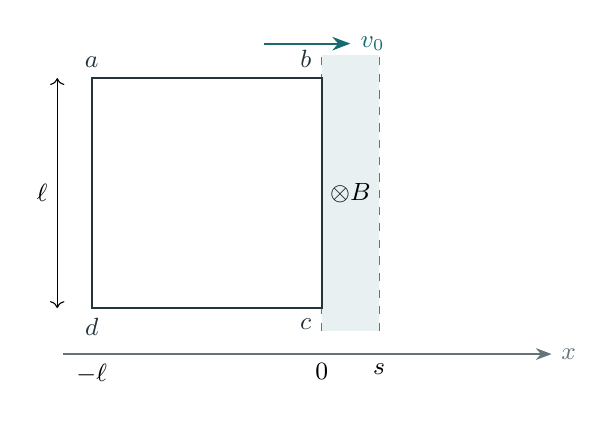
\begin{tikzpicture}[scale=.73]

\fill[accent!10](0,-.4) rectangle(1,4.4);\draw[guide](0,-.4)--(0,4.4) (1,-.4)--(1,4.4);
\draw[object](-4,0) node[below]{$d$}--(0,0) node[below left]{$c$}--(0,4) node[above left]{$b$}--(-4,4) node[above]{$a$}--cycle;
\draw[motion](-1,4.6)--(.5,4.6) node[right]{$v_0$};\node at(.5,2){$\otimes B$};
\draw[axis](-4.5,-.8)--(4,-.8) node[right]{$x$};\node[below] at(0,-.8){$0$};\node[below] at(1,-.8){$s$};\node[below] at(-4,-.8){$-\ell$};
\draw[<->](-4.6,0)--(-4.6,4) node[midway,left]{$\ell$};

\end{tikzpicture}\figcaption{图电3.18\quad 正方形框的边长为$\ell=4s$，初始右边$bc$在场区入口。}\end{minipage}\end{center}

\workarea

\clearpage

\pdfbookmark[2]{第 19 题 由持久电流衰减估计电阻率上限}{q19}

\section*{第 19 题\quad 由持久电流衰减估计电阻率上限}\label{q:19}

一个细圆环的圆环半径$R_c=0.10\,\mathrm m$，导线截面为半径$a=1.0\times10^{-3}\,\mathrm m$的圆。环内持久电流初值$I_0=100\,\mathrm A$，一年后电流的减少量小于$10^{-6}\,\mathrm A$。把圆环视为具有恒定微小电阻和自感的孤立回路，不受外磁通变化影响。取一年$T=3.1536\times10^7\,\mathrm s$，$\mu_0=4\pi\times10^{-7}\,\mathrm{H/m}$，估计导体电阻率的上限数量级，并说明电感估算对结论的影响。

\begin{center}\begin{minipage}{.98\linewidth}\centering
\begin{tikzpicture}[scale=.85]

\draw[object] (0,0) circle(2);\draw[object] (0,0) circle(1.85);\draw[axis] (0,0)--(0,1.925) node[midway,left]{$R_c$};
\draw[motion] (30:2.2) arc(30:100:2.2) node[above]{$I_0$};\draw[guide] (1.95,0)--(4.2,0);
\draw[object] (5,0) circle(.7);\draw[axis] (5,0)--(5.7,0) node[midway,above]{$a$};\node at(5,-1.2){导线截面放大};

\end{tikzpicture}\figcaption{图电3.19\quad 大环半径与导线截面半径分别参与长度与截面积。}\end{minipage}\end{center}

\workarea

\clearpage

\pdfbookmark[2]{第 20 题 恒流双线分离时的磁能与机械功}{q20}

\section*{第 20 题\quad 恒流双线分离时的磁能与机械功}\label{q:20}

两根半径$a=1.0\,\mathrm{cm}$的平行长直圆柱导线，轴距$d=20\,\mathrm{cm}$，分别通大小均为$I=20\,\mathrm A$、方向相反的恒定电流。忽略端部效应，以$a/d$为小量求两线系统单位长度的外自感。随后缓慢将轴距增加到$d'=40\,\mathrm{cm}$，电流由电源维持不变，求单位长度的磁力功、磁能增量及电源额外提供的能量，说明三者关系。不计导线内部磁能，普通电阻耗散作为不变背景另行扣除。

\begin{center}\begin{minipage}{.98\linewidth}\centering
\begin{tikzpicture}[scale=.85]

\draw[object] (0,0) circle(.2);\node at(0,0){$\odot$};\draw[object] (4,0) circle(.2);\node at(4,0){$\otimes$};
\node[above] at(0,.5){$I$};\node[above] at(4,.5){$I$};\draw[<->] (0,-.8)--(4,-.8) node[midway,below]{$d\to d'$};
\draw[guide](.14,.14)--(.7,.6) node[right]{$a$};\draw[force] (-.5,0)--(-1.5,0);\draw[force] (4.5,0)--(5.5,0);
\node at(2,1.5){截面图：反向恒流相互排斥};

\end{tikzpicture}\figcaption{图电3.20\quad 缓慢增大轴距，电源维持电流不变。}\end{minipage}\end{center}

\workarea

\clearpage

\pdfbookmark[2]{第 21 题 柔性线圈测量磁场线积分}{q21}

\section*{第 21 题\quad 柔性线圈测量磁场线积分}\label{q:21}

在横截面积为$S$、不导磁的柔性细带上均匀绕制线圈，单位弧长$n$匝，沿空间曲线从$a$延伸到$b$。线圈两端经紧贴并行的引线接冲击电流计，回路总电阻为$R$；引线额外链接磁通忽略。初始外磁场为$\vect H_0$，随后产生该磁场的电流降为零。细带固定，各处磁场在小截面内可视为均匀，测得完整瞬态通过电流计的有向电量$q$，初、末回路电流均为零。证明适当选定绕向后，$\int_a^b\vect H_0\cdot\dd\vect l=Rq/(\mu_0nS)$，讨论是否必须忽略自感。

\begin{center}\begin{minipage}{.98\linewidth}\centering
\begin{tikzpicture}[scale=.85]

\draw[guide,very thick] (0,0) .. controls (2,3) and(4,-1).. (6,2);
\foreach \x/\y/\ang in {0/0/-35,.6/.65/-30,1.2/1.1/-20,1.8/1.25/0,2.4/1.2/15,3/1.05/20,3.6/.98/0,4.2/1.05/-15,4.8/1.3/-25,5.4/1.65/-30,6/2/-35}{\draw[object,rotate around={\ang:(\x,\y)}] (\x,\y) ellipse(.13 and .35);}
\node[left] at(0,0){$a$};\node[right] at(6,2){$b$};\draw[object] (0,0)--(0,-1.3)--(6,-1.3)--(6,2);\node[fill=white] at(3,-1.3){冲击电流计};
\draw[motion] (4,2.5)--(5,3.2) node[right]{$\vect H_0$};\node at(3,-2){回引线紧贴布置，额外磁通忽略};

\end{tikzpicture}\figcaption{图电3.21\quad 线圈沿柔性细带的空间路径分布；下方连接仅示意电接法。}\end{minipage}\end{center}

\workarea

\clearpage

\pdfbookmark[2]{第 22 题 相切圆环与反向双直线电流的互感}{q22}

\section*{第 22 题\quad 相切圆环与反向双直线电流的互感}\label{q:22}

两根无限细长直导线平行，相距$2a$，通大小相等、方向相反的电流$I$。半径$a$的细圆环处在两线共面区域，圆心位于两线中间，并与两线相切；相切处绝缘，所有导线不电接触。求双直线电流回路与圆环之间互感的大小。理想零线径产生的切点磁场奇异性按极限积分处理，忽略圆环自身磁场。

\begin{center}\begin{minipage}{.98\linewidth}\centering
\begin{tikzpicture}[scale=.85]

\draw[object] (0,-2.5)--(0,2.5) (4,-2.5)--(4,2.5);\draw[object] (2,0) circle(2);
\draw[motion] (-.35,-1)--(-.35,1) node[above]{$I$};\draw[motion] (4.35,1)--(4.35,-1) node[below]{$I$};
\draw[axis] (2,0)--(2,2) node[midway,right]{$a$};\draw[<->] (0,-2.9)--(4,-2.9) node[midway,below]{$2a$};
\node at(2,-.7){$\otimes B$};\node at(6,0){切点绝缘};

\end{tikzpicture}\figcaption{图电3.22\quad 两线的反向电流在圆内形成同向磁场。}\end{minipage}\end{center}

\workarea

\clearpage

\pdfbookmark[2]{第 23 题 互感线圈的短接、串联与并联}{q23}

\section*{第 23 题\quad 互感线圈的短接、串联与并联}\label{q:23}

两个线性无损线圈自感为$L_1,L_2>0$，互感大小为$M\ge0$。用同名端的点号约定：两个参考电流都流入点端时，互感项取正。分别求：（1）第二线圈短接，从第一线圈两端看入的等效电感；（2）两线圈顺接串联的等效电感，及反接一线圈的结果；（3）两线圈反点号并联，即输入节点$A$接第一线圈点端和第二线圈非点端，节点$B$接另外两端时的等效电感，及翻转一线圈后的结果。证明$M^2\le L_1L_2$，并讨论完全耦合的退化情形。初始电流取零，除讨论退化时外先设$M^2<L_1L_2$。

\begin{center}\begin{minipage}{.98\linewidth}\centering
\begin{tikzpicture}[scale=.77]
\node at(1,3){副边短接};\draw[object] (0,0)--(0,0.4);\draw[object] (0,1.6)--(0,2);\draw[object] (0,0.4) arc(-90:90:.15) arc(-90:90:.15) arc(-90:90:.15) arc(-90:90:.15);\node[left] at(-0.12,1){$L_1$};\fill (-0.18,1.8) circle(2pt);\draw[object] (2,0)--(2,0.4);\draw[object] (2,1.6)--(2,2);\draw[object] (2,0.4) arc(-90:90:.15) arc(-90:90:.15) arc(-90:90:.15) arc(-90:90:.15);\node[left] at(1.88,1){$L_2$};\fill (1.82,1.8) circle(2pt);\draw[object] (2,0)--(3,0)--(3,2)--(2,2);\node[left] at(0,2){$A$};\node[left] at(0,0){$B$};\node at(5.5,3){顺接串联};\draw[object] (4.5,0)--(4.5,0.4);\draw[object] (4.5,1.6)--(4.5,2);\draw[object] (4.5,0.4) arc(-90:90:.15) arc(-90:90:.15) arc(-90:90:.15) arc(-90:90:.15);\node[left] at(4.38,1){$L_1$};\fill (4.32,1.8) circle(2pt);\draw[object] (6.5,0)--(6.5,0.4);\draw[object] (6.5,1.6)--(6.5,2);\draw[object] (6.5,0.4) arc(-90:90:.15) arc(-90:90:.15) arc(-90:90:.15) arc(-90:90:.15);\node[left] at(6.38,1){$L_2$};\fill (6.32,1.8) circle(2pt);\draw[object] (4.5,0)--(5.5,0)--(5.5,2)--(6.5,2);\node[left] at(4.5,2){$A$};\node[right] at(6.5,0){$B$};\node at(10,3){反点号并联};\draw[object] (9,0)--(9,0.4);\draw[object] (9,1.6)--(9,2);\draw[object] (9,0.4) arc(-90:90:.15) arc(-90:90:.15) arc(-90:90:.15) arc(-90:90:.15);\node[left] at(8.88,1){$L_1$};\fill (8.82,1.8) circle(2pt);\draw[object] (11,0)--(11,0.4);\draw[object] (11,1.6)--(11,2);\draw[object] (11,0.4) arc(-90:90:.15) arc(-90:90:.15) arc(-90:90:.15) arc(-90:90:.15);\node[left] at(10.88,1){$L_2$};\fill (10.82,0.2) circle(2pt);\draw[object] (9,2)--(11,2) (9,0)--(11,0);\node[above] at(10,2){$A$};\node[below] at(10,0){$B$};
\end{tikzpicture}\figcaption{图电3.23\quad 点号给出同名端；连接线和端点决定各接法的互感符号。}\end{minipage}\end{center}

\workarea

\end{document}
